\documentclass{article}
\usepackage{tikz}
\usepackage{amsmath}
\usepackage{bm}
\usepackage{scalerel}
\usepackage{pgfplots}
\usepackage{mathpazo}
\pgfplotsset{width=7cm,compat=1.8}
\usetikzlibrary{patterns}
\usetikzlibrary{arrows,shapes,calc}
\usetikzlibrary{external}
\tikzset{external/system call={pdflatex \tikzexternalcheckshellescape -halt-on-error
        -interaction=batchmode -jobname "\image" "\texsource" && %  or ;
pdftops -eps "\image".pdf}}
\tikzexternalize




\begin{document}
	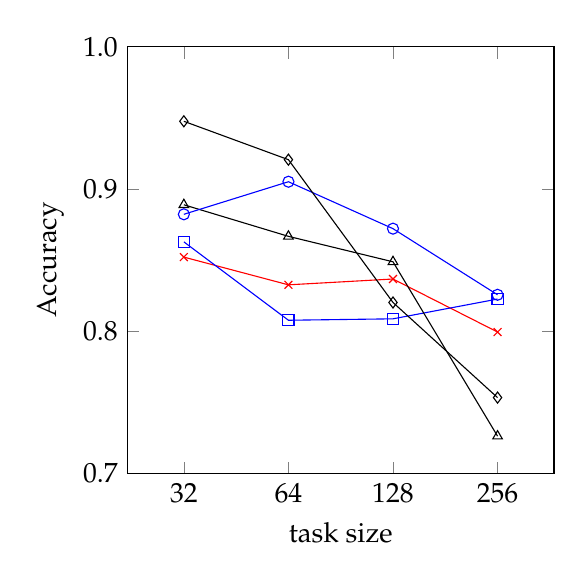
\begin{tikzpicture}
	\definecolor{lssfre}{HTML}{fccde5}
	\definecolor{lssemb}{HTML}{bc80bd}
	\definecolor{lsscon}{HTML}{bebada}
	\definecolor{wj}{HTML}{fb8072}
	\definecolor{impr}{HTML}{80b1d3}
	\definecolor{cs}{HTML}{fdb462}
	\definecolor{cset}{HTML}{b3de69}
	\definecolor{jsub}{HTML}{8dd3c7}
	\definecolor{sumrdf}{HTML}{ffffb3}
	\definecolor{bsk}{HTML}{d9d9d9}
	\centering
	\begin{axis}[
	height=7cm, width=7cm,
	%enlarge y limits={value=.1,upper},
	ymin=0.7, ymax=1.0,
	%ymode=log,
	%log origin=infty,
	enlarge x limits=true,
	legend style={
		at={(0.5, 1.2)},
		anchor=north,
		legend columns=3
	},
	ylabel={Accuracy},
	ytick={0.7, 0.8, 0.9, 1.0},
	yticklabels={$0.7$, $0.8$, $0.9$, $1.0$},
	xmin=0.8, xmax = 4.2,
	xtick={1, 2, 3, 4},
	xticklabels={32, 64, 128, 256},
	xlabel={task size},
	%symbolic x coords={
	%	Facebook, Gowalla, WikiConflict, Google, DBLP, Berkstan, Youtube, Petster, Flickr,
	%Indochina },
	%xtick=data,
	]


	% rand
 	\addplot [color=red,mark=x] coordinates {
	(1, 0.8521)
	(2, 0.8326)
	(3, 0.8367)
	(4, 0.7994)		
    };
    % homo-g
 	\addplot [color=blue,mark=square] coordinates {
	(1, 0.8628)
	(2, 0.8077)
	(3, 0.8087)
	(4, 0.8226)
	};
    
   	% homo-p
 	\addplot [color=black,mark=triangle] coordinates {
	(1, 0.8889)
	(2, 0.8667)
	(3, 0.8488)
	(4, 0.7262)
    };
    
    % hyrbid-g
 	\addplot [color=blue,mark=o] coordinates {
	(1, 0.8822)
	(2, 0.9051)
	(3, 0.8721)
	(4, 0.8256)
    };
    
    % hyrbid-p
 	\addplot [color=black,mark=diamond] coordinates {
	(1, 0.9476)
	(2, 0.9206)
	(3, 0.8202)
	(4, 0.7533)
    };



	
	\legend{
%		    \large $\texttt{Rand}$,
%		    \large $\texttt{Homo.~g}$,
%		    \large $\texttt{Homo.~p}$,
%		    \large $\texttt{Hyb.~g}$,
%		    \large $\texttt{Hyb.~p}$
	        }
	\end{axis}
	\end{tikzpicture}

\end{document}

